\chapter{Preliminary Examination}
Cloud detection from satellite photos is critical for a variety of purposes, including weather forecasting, emergency management, and climate research. This report presents a preliminary examination of a project aimed at developing an accurate and efficient cloud detection algorithm from satellite images. To detect clouds in satellite photos, the research was employed machine learning models and image processing techniques. This objective was been accomplished by semantic segmentation and remote sensing using the U-Net architecture. Satellite pictures were been created using the Landsat-8 dataset. 

\section{Literature Review}

The research about cloud detection algorithms likely started in the 1990s. Some studies have been examined and five of them information are given below. 


\begin{itemize}
    \item \cite{fifth} The research was published in 10 October 2017. Model was built on deep learning system to categorize cloud and snow at the pixel level using fully convolutional neural networks. To learn deep patterns, a specialized fully convolutional network was implemented. Then, to integrate low-level spatial and high-level semantic information at the same time, a multiscale prediction technique was used.  50 Gaofen \#1 satellite images with the resolution of 16 m, where each image is with a size of 13400×12000 pixels was used for evaluate the model. Precision, recall and mIOU have been used for measuring success. According to research, precision, recall and mIOU were calculated as 92.4, 91.5, 90.6 respectively.

    \item \cite{fourth} The research was published in 14 November 2018. It mostly dwells on small and thin cloud detection. The model has been trained and tested on the special dataset gathered from the G1 satellite. The dataset includes 100 testing and 38 training images. After dividing the images into patches, 206000 patches has gained. The model was designed with NSS and Gabor features. Three steps take place. First, segmentation is done first using the SLIC technique. Then, The uncertain superpixels are then divided into potential  thin clouds, thick clouds and nonclouds using the NSS features. Lastly, Gabor features are input to an SVM that can distinguish between cloudy and snowy regions. Training and validation patches are 8400 in total. Testing patches are 9200. Precision and recall values have been used for measuring success. Precision and recall were calculated 91.61, 86.39 respectively.

    \item \cite{second} The research was published in  May 2019. CNN based on segNet was used in the research. The algorithm contains 13 convolution layer and 13 deconvolution layer. The model was trained and evaluated using 32 Landsat 8 images and 38 Landsat 7 images. \%60 of the dataset was used for training, \%10 was used for backpropogation and \%30 was used for testing. Algorithm compared with CFMask and the result of this, the overall accuracies are improved from 89.88 and 84.58 to 95.26 and 95.47 for the Landsat 7 and Landsat 8 images.

    \item \cite{first} The research was published in January 2019. The purpose of the research is prevent the incorrect cloud detection  and make algorithm efficient for the snowy areas. To achieve this RS-Net model was developed. The model was trained and evaluated using the Landsat 8 Biome and SPARCS datasets. Landsat 8 Biome dataset has a size of 195 GB and contains 96 Landsat 8 scenes. Dataset includes 8 different biome and they divided into 4 classes, namely ‘cloud’, ‘thin cloud’, ‘cloud shadow’, and ‘clear’.  Landsat 8 SPARCS dataset has size of 1.6 GB and consists of 80 1000 x 1000 pixels scenes. It is divided into 7 classes, namely ‘cloud shadow’, ‘cloud shadow over water’, ‘water’, ‘snow’, ‘land’, ‘cloud’, and ‘flooded’. Two dataset was merged and SPARCS dataset is converted to cloud, shadow and clear classes. Algorithm was evaluated and tested with combinations of two dataset. Accuracy, precision, and recall metrics have been used for measuring success. The best results are become by using Sparcs dataset for training and testing the model. Accuracy and F1 score were calculated 94.54, 85.59 respectively.

    \item  C: \cite{third} The research published in 2021. The model has generated by using U-Net on Landsat 8 satellite images. In the dataset, 38 images have been divided into 384*384 patches. The patches are split into training, validation, and testing. Training and validation patches are 8400 in total. Testing patches are 9200. Precision  and recall  values have been used for measuring success. Precision and recall values were calculated \%85.28, \%83.23 respectively.
\end{itemize}
\hfill \break
The abstracts of the all researches are given below at Figure \ref{lit_rew}.
\begin{figure}[htp]
    \centering
    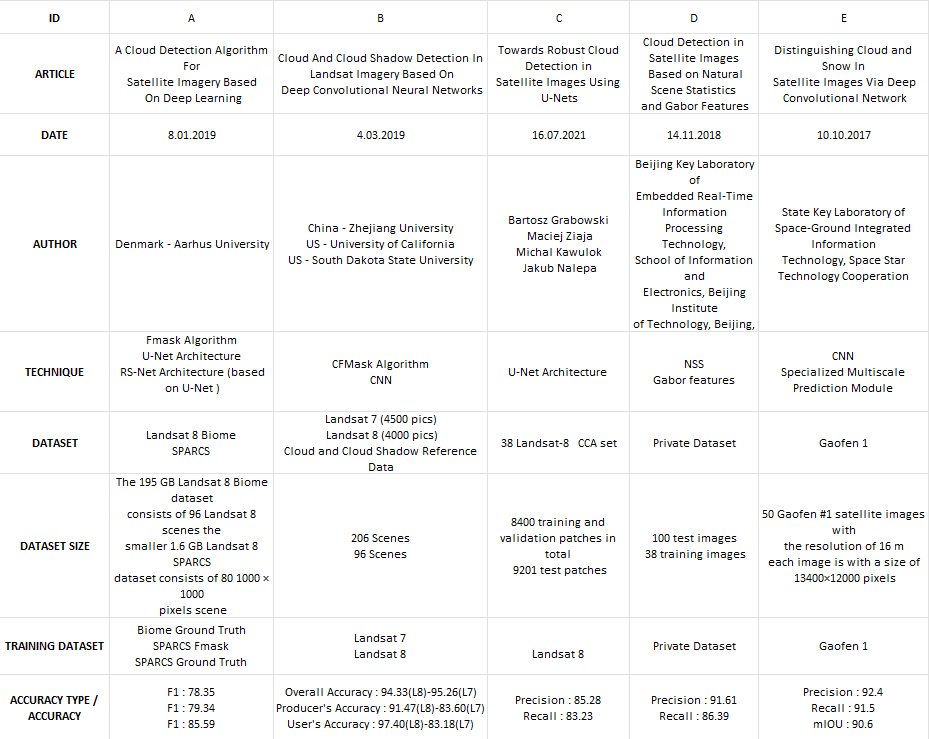
\includegraphics[width=15cm]{projectChapters/images/litareture.png}
    \caption{Abstracts of All Researches}
    \label{lit_rew}
\end{figure}

A: \cite{first}, B: \cite{second}, C: \cite{third}, D: \cite{fourth}, E: \cite{fifth}
